\documentclass[areasetadvanced]{scrartcl}

\usepackage[utf8]{inputenc}
\usepackage[T2A]{fontenc}
\usepackage[english,russian]{babel}
\usepackage[scaled=0.92]{DejaVuSansMono}
\usepackage{xcolor}

\usepackage[footskip=1cm,left=25mm, right=15mm, top=20mm, bottom=20mm]{geometry}
\usepackage{setspace}
\usepackage{amsmath, amssymb} 
\usepackage{graphicx}
\usepackage{tikz}
\usetikzlibrary{arrows.meta}
\usepackage{float}
\usepackage{dashrule}
\usepackage{fancyhdr} 
\usepackage{hyperref}
\hypersetup{colorlinks=true,linkcolor=blue,urlcolor=blue,citecolor=blue}
\usepackage{parskip}
\usepackage{textcomp, enumitem}
\usepackage{indentfirst}
\usepackage{graphicx}
\usepackage{algorithm}
\usepackage{xltabular}
\usepackage{xtab}
\usepackage{algpseudocode}
\usepackage{array} 
\usepackage{geometry}
\usepackage{afterpage}
\usepackage{minted}
\setcounter{secnumdepth}{3} 
\setcounter{tocdepth}{3}    
\usepackage{listings}
\usepackage{fvextra}
\usepackage{booktabs}
\usepackage{paracol} % параллельные колонки (левая/правая)

\newcommand{\icon}[1]{\includegraphics[height=1.2em]{#1}}
% Ссылка на приложение по букве (якорь задаётся \phantomsection\label у заголовка приложения)
\newcommand{\appref}[2]{\hyperref[#1]{#2}}

\tikzstyle{block} = [rectangle, rounded corners, minimum width=3cm, minimum height=1cm, text centered, draw=black, fill=lightgray]

\setkomafont{sectioning}{\normalfont\bfseries} 
\setkomafont{section}{\normalfont\Large\bfseries}
\setkomafont{subsection}{\normalfont\large\bfseries}
\setkomafont{subsubsection}{\normalfont\large\bfseries}
\setkomafont{paragraph}{\normalfont\large\bfseries} 
\newcommand{\twosideheading}[2]{%
  \noindent
  \begin{minipage}[t]{0.5\textwidth}\raggedright\small #1\end{minipage}%
  \begin{minipage}[t]{0.5\textwidth}\raggedleft\Large\bfseries #2\end{minipage}\\[-0.2em]
  \hrule
  \vspace{0.8em}
}
\lstset{
  language=Haskell,
  basicstyle=\ttfamily\small,
  keywordstyle=\color{blue}\bfseries,
  stringstyle=\color{red},
  commentstyle=\color{green!70!black},
  numbers=left,
  numberstyle=\tiny,
  stepnumber=1,
  numbersep=10pt,
  showstringspaces=false,
  breaklines=true,
  frame=single
}

\lstdefinelanguage{Lua}{
    keywords={function, end, if, then, else, elseif, for, while, do, repeat, until, break, return, local, and, or, not, true, false, nil},
    keywordstyle=\color{blue}\bfseries,
    stringstyle=\color{red},
    commentstyle=\color{green!70!black},
    morestring=[s]{"}{"},
    morestring=[s]{'}{'},
    morecomment=[l]{-},
    morecomment=[s]{-[[}{]]},
    basicstyle=\ttfamily\small,
    numbers=left,
    numberstyle=\tiny,
    stepnumber=1,
    numbersep=10pt,
    showstringspaces=false,
    breaklines=true,
    frame=single
}

\lstdefinestyle{py}{
    language=Python,
    basicstyle=\ttfamily\small,
    keywordstyle=\color{blue}\bfseries,
    stringstyle=\color{red},
    commentstyle=\color{green!70!black},
    numbers=left,
    numberstyle=\tiny,
    stepnumber=1,
    numbersep=10pt,
    showstringspaces=false,
    breaklines=true,
    frame=single
}

\setlength{\parindent}{1.25cm}
\setcounter{tocdepth}{3}

\lstdefinestyle{appendixcode}{
    basicstyle=\ttfamily\footnotesize,
    numbers=left,
    numberstyle=\tiny\color{gray},
    numbersep=6pt,
    breaklines=true,
    breakatwhitespace=true,
    frame=single,
    tabsize=2,
    showstringspaces=false,
    xleftmargin=1.5em,
    framexleftmargin=1.2em
}
\lstdefinestyle{appendixshell}{
    style=appendixcode,
    language=bash,
    keywordstyle=\color{blue!70!black}
}

\begin{document}
\sloppy
	\thispagestyle{empty}
	\begin{center}
	\large{МИНОБРНАУКИ РОССИИ} \par
	\vspace{0.3cm}
	\normalsize
	{ФЕДЕРАЛЬНОЕ ГОСУДАРСТВЕННОЕ АВТОНОМНОЕ ОБРАЗОВАТЕЛЬНОЕ УЧРЕЖДЕНИЕ ВЫСШЕГО ОБРАЗОВАНИЯ} \par
	\vspace{0.3cm}
	\textbf{САНКТ-ПЕТЕРБУРГСКИЙ ПОЛИТЕХНИЧЕСКИЙ}
	\textbf{УНИВЕРСИТЕТ ПЕТРА ВЕЛИКОГО} \par
	\vspace{0.3cm}
	{Институт компьютерных наук и кибербезопасности}\par
	{Высшая школа технологий искусственного интеллекта}\par
\end{center}
\vfill
\begin{center}
	{\huge Отчёт о выполнении лабораторных работ}\par
	%\vspace{0.1cm}
    \huge {по дисциплине:}\par
    \vspace{0.3cm}
	\Huge \textbf{Высокоскоростные сетевые технологии суперкомпьютеров}\par
\end{center}
\vfill
\begin{flushleft}
	Студент: \hspace{1.8cm} \rule[0pt]{2.5cm}{0.5pt}\hfill Салимли Айзек Мухтар Оглы\par
	\vspace{1.5cm}
	Преподаватель: \hspace{0.55cm} \rule[0pt]{2.5cm}{0.5pt}\hfill  Курочкин Михаил Александрович
\end{flushleft}
\vspace{0.5cm}
\begin{flushright}
	\guillemotleft \rule[0pt]{0.8cm}{0.5pt}\guillemotright \rule[0pt]{2cm}{0.5pt} 20\rule[0pt]{0.5cm}{0.5pt} г.
\end{flushright}
\vfill
\begin{center}
	Санкт-Петербург, 2026
\end{center}

\newpage
\tableofcontents

\newpage
\section*{Введение}
\addcontentsline{toc}{section}{Введение}

Современные вычислительные системы опираются на несколько взаимодополняющих моделей параллелизма. Графические ускорители с архитектурой массового параллелизма позволяют задействовать тысячи нитей при обработке регулярных численных структур; в экосистеме NVIDIA для этого широко применяется технология CUDA. Для многопроцессорных и многомашинных конфигураций стандартным средством координации выступает интерфейс MPI (Message Passing Interface), обеспечивающий обмен сообщениями между процессами, в том числе при работе на вычислительном кластере.

Оценка практической производительности суперкомпьютеров и вычислительных узлов традиционно опирается на решение систем линейных алгебраических уравнений; этой цели служит тест LINPACK, результаты которого выражаются в показателях вроде пиковой и достигнутой производительности (Rmax, число операций с плавающей точкой в единицу времени).

Цель работы - изучить подходы к оценке производительности и сопоставить различные технологии параллельного программирования на примере двух задач.

В \textbf{первой лабораторной работе} рассматривается итерационное решение СЛАУ методом Якоби на GPU с использованием CUDA; полученные времена сопоставляются с запуском эталонного теста Intel LINPACK на CPU узла с графическим ускорителем. Таким образом, сочетаются исследование характерного для HPC и практика разработки CUDA-ядра для плотной линейной алгебры.

Во \textbf{второй лабораторной работе} решается прикладная задача построения матрицы алгебраических дополнений заданной квадратной матрицы. Требуется реализовать распределённый вариант на кластере средствами MPI, сопоставить его с исходной CUDA-реализацией и проанализировать зависимость времени выполнения от числа задействованных процессов и узлов.

Эксперименты проводились на ресурсах суперкомпьютерного центра «Политехнический»; для удалённого доступа использовались учётные данные, выданные для работы в СКЦ.

\textbf{В качестве пользователя: tm3u20.} Вход на кластер выполнялся через узел доступа \texttt{login1.hpc.spbstu.ru} с использованием SSH-ключа.

\newpage
\section{Лабораторная работа №1}

\subsection{Постановка задачи}

В рамках первого задания требовалось исследовать производительность вы-
числительной системы при решении плотной системы линейных алгебраических
уравнений и сопоставить результаты собственной реализации с эталонным тестом
LINPACK. Для достижения этой цели были поставлены следующие задачи:
\begin{itemize}
\item изучить подходы к оценке производительности вычислительных систем;
\item разработать собственную CUDA-реализацию LINPACK-подобного теста;
\item выполнить экспериментальные запуски на вычислительном узле СКЦ Поли-
технический;
\item сравнить результаты собственной программы и стандартного Intel LINPACK.
\end{itemize}

\subsection{Математическое описание}

Тест LINPACK применяется для оценки производительности вычислительных систем при решении плотной системы линейных уравнений. Рассматривается задача
\begin{equation}
    A x = b,
\end{equation}
где $A \in \mathbb{R}^{n \times n}$ - плотная квадратная матрица, $x \in \mathbb{R}^{n}$ - искомый вектор решения, $b \in \mathbb{R}^{n}$ - вектор правой части.

В классическом варианте LINPACK обычно применяются прямые методы, основанные на LU-разложении. В собственной реализации для первого задания использован итерационный метод Якоби, так как он хорошо распараллеливается на GPU: каждая строка матрицы может обрабатываться независимо.

Для метода Якоби очередное приближение вычисляется по формуле
\begin{equation}
    x_i^{(k+1)} = \frac{1}{a_{ii}} \left( b_i - \sum\limits_{j \ne i} a_{ij} x_j^{(k)} \right), \quad i = 1, 2, \dots, n.
\end{equation}

Критерий остановки выбран в виде
\begin{equation}
    \max_i \left| x_i^{(k+1)} - x_i^{(k)} \right| \le \varepsilon.
\end{equation}

Чтобы обеспечить сходимость метода, в программе формируется строго диагонально доминирующая матрица. Для контроля качества решения дополнительно вычисляются:
\begin{equation}
    \| A x - b \|_{\infty},
\end{equation}
\begin{equation}
    \| x - x_{true} \|_{\infty},
\end{equation}
где $x_{true}$ - заранее известное опорное решение, использованное при построении тестовой системы.

Для приближённой оценки производительности используется LINPACK-подобная метрика
\begin{equation}
    R = \frac{\frac{2}{3} n^3}{t},
\end{equation}
где $t$ - время решения, измеренное в секундах. В отчёте далее используется величина $R$ в GFLOPS.

\subsection{Особенности реализации}

Собственная программа реализована на CUDA C++ (файл \texttt{task\_1/src/main.cu}). Принятые решения:
\begin{itemize}
  \item сетка потоков одномерная: каждому индексу строки $i$ соответствует ровно один поток CUDA, вычисляющий компоненту $x_i^{(k+1)}$ по формуле Якоби;
  \item матрица $A$, векторы $b$, $x$ и служебные буферы размещаются в памяти GPU; итерации выполняются с чередованием буферов \texttt{d\_x\_old} и \texttt{d\_x\_new} без лишних копирований на хост;
  \item флаг сходимости хранится в глобальной памяти устройства; перед шагом Якоби он устанавливается в «сошлось», затем ядро \texttt{jacobi\_iteration} при нарушении условия $|x_i^{(k+1)}-x_i^{(k)}|>\varepsilon$ сбрасывает его через \texttt{atomicAnd};
  \item после остановки итераций на CPU вычисляются $\|Ax-b\|_\infty$ и $\|x-x_{\mathrm{true}}\|_\infty$; производительность оценивается как $R=\frac{2}{3}n^3/t$ (GFLOPS);
  \item для снижения дисперсии замеров поддерживаются прогрев (\texttt{-warmup}) и несколько повторов (\texttt{-repeat}) с выбором лучшего времени; результаты могут выводиться в CSV (\texttt{-csv}).
\end{itemize}
Реализация не эквивалентна классическому LU-LINPACK, но решает ту же прикладную задачу оценки производительности при работе с плотной СЛАУ на GPU. Полный исходный текст приведён в приложении~\appref{app:t1-main}{А}.

\subsection{Сборка и запуск собственного теста (CUDA)}

Исходные материалы располагались в каталоге проекта \texttt{task\_1}. Сборка и запуск CUDA-варианта выполнялись сценарием \texttt{task\_1/scripts/run\_cuda.slurm}: загружаются модули \texttt{compiler/gcc/11} и \texttt{nvidia/cuda/11.6u2}, вызывается \texttt{scripts/build.sh} (сборка \texttt{nvcc}, текст - приложение~\appref{app:t1-build}{Д}), бинарь \texttt{bin/linpack\_cuda} запускается с параметрами серии размеров $N=1000,1500,\ldots,3500$, $\varepsilon=10^{-6}$, записью CSV в \texttt{results/task1-cuda-<JOBID>.csv}. Перед подачей задания скрипту выдаётся право на исполнение (\texttt{chmod +x run\_cuda.slurm}). Текст сценария - приложение~\appref{app:t1-slurm-cuda}{Б}.

Эталонный Intel LINPACK (исполняемый файл \texttt{xlinpack\_xeon64} из дистрибутива Intel) запускался сценарием \texttt{task\_1/scripts/run\_intel\_linpack.slurm} (приложение~\appref{app:t1-slurm-intel}{В}) на разделе \texttt{tornado} с \texttt{-cpus-per-task=56}, переменными \texttt{OMP\_NUM\_THREADS} и \texttt{MKL\_NUM\_THREADS}, согласованными с SLURM. Входной файл \texttt{task\_1/intel/lininput\_report\_xeon64} (приложение~\appref{app:t1-lininput}{Г}) задаёт те же шесть размеров задачи и параметры повторных прогонов, что и для CUDA.

\subsection{Результаты эксперимента}

Как было сказано ранее во введении, для подтверждения собственной реализации все действия выполнены пользователем tm3u20.

Ниже на рисунках \ref{fig:login} - \ref{fig:job_info_3} приведены результаты эксперимента. 

\begin{figure}[H]
    \centering
    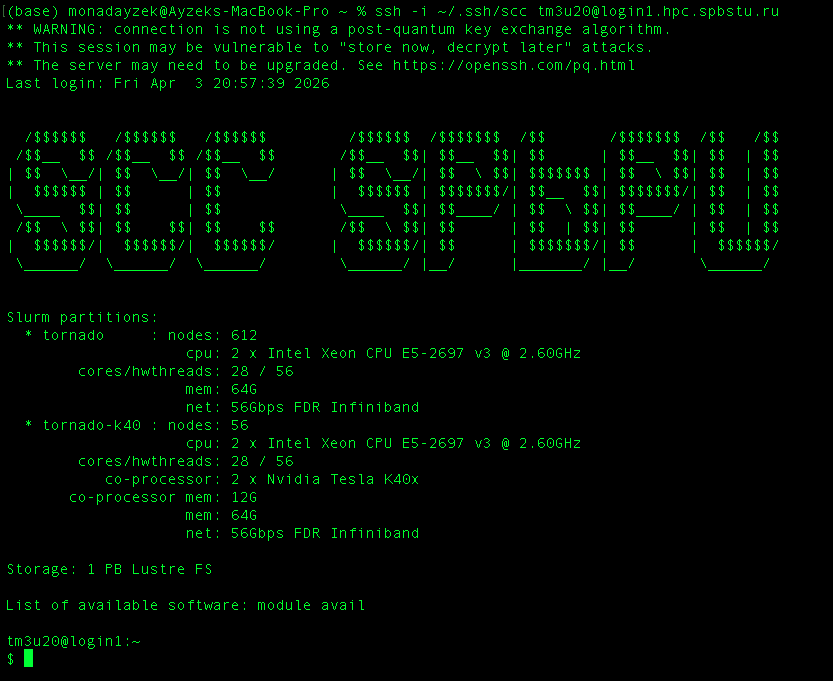
\includegraphics[width=0.8\textwidth]{img/1_login_scc.png}
    \caption{Подключение к кластеру пользователем tm3u20}
    \label{fig:login}
\end{figure}

После подключения к кластеру, для удобства была создана директория \texttt{supercomputers/my} для работы с заданиями:

\begin{figure}[H]
    \centering
    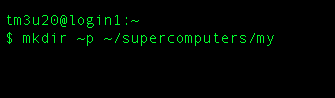
\includegraphics[width=0.8\textwidth]{img/2_create_folder.png}
    \caption{Создание директории \texttt{supercomputers/my}}
    \label{fig:create_task_1_dir}
\end{figure}

Ниже показан результат создания рабочей директории:

\begin{figure}[H]
    \centering
    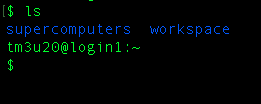
\includegraphics[width=0.8\textwidth]{img/3_check_folder.png}
    \caption{Результат создания рабочей директории}
    \label{fig:create_task_1_dir_result}
\end{figure}

Далее код написанный на собственном компьютере был скопирован в директорию с помощью утилиты \texttt{scp}.

Далее перед запуском необходимо дать права на выполнение скрипта путем выполнения команды:
\begin{lstlisting}[caption=Выдача прав на выполнение скрипта, language=bash]
    chmod +x run_cuda.slurm
\end{lstlisting}

Ниже показана команда выдачи прав и выполнение скрипта:

\begin{figure}[H]
    \centering
    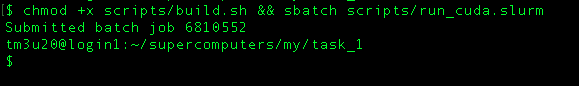
\includegraphics[width=0.8\textwidth]{img/4_chmod_and_run.png}
    \caption{Выдача прав на выполнение скрипта}
    \label{fig:give_permissions}
\end{figure}

Из вывода видно что задача запустилась в очереди с ID (идентификатором) = 6810552. 

Готовность задачи можно проверить с помощью команды:
\begin{lstlisting}[caption=Проверка готовности задачи, language=bash]
    squeue -j 6810552
\end{lstlisting}

Ниже показан результат проверки готовности задачи:

\begin{figure}[H]
    \centering
    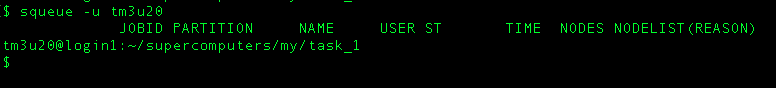
\includegraphics[width=0.8\textwidth]{img/5_job_done.png}
    \caption{Проверка готовности задачи}
    \label{fig:check_job_status}
\end{figure}

Из вывода видно, что задач в процессе выполнения нет. Что означает что задача выполнена.

Далее на рисунке \ref{fig:job_info_1} - \ref{fig:job_info_3} показан вывод задачи:

\begin{figure}[H]
    \centering
    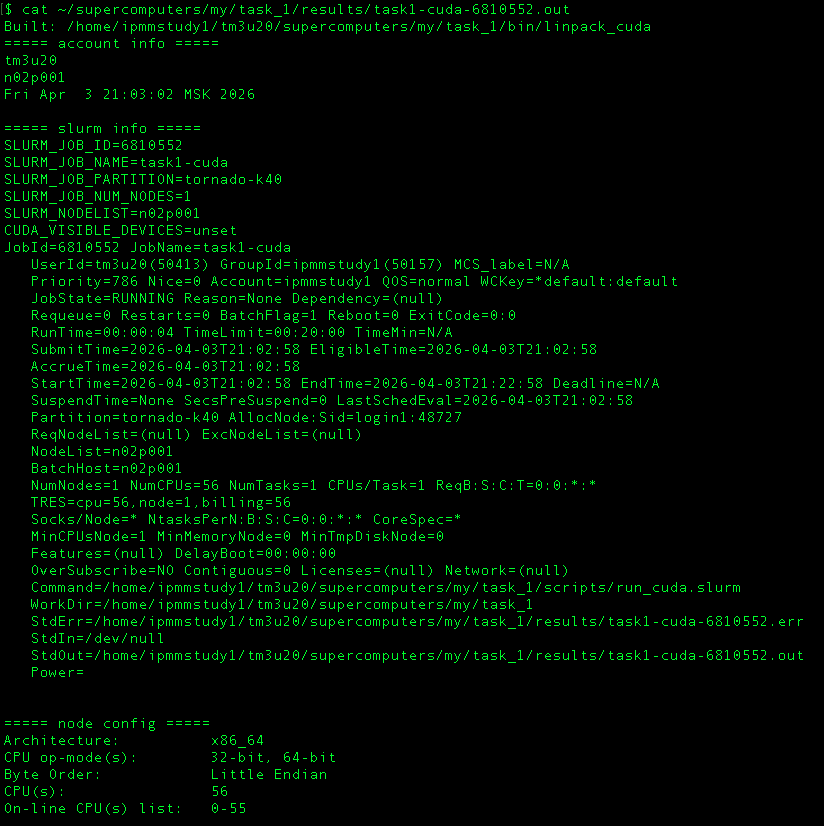
\includegraphics[width=0.8\textwidth]{img/6_job_info_1.png}
    \caption{Вывод задачи}
    \label{fig:job_info_1}
\end{figure}

\begin{figure}[H]
    \centering
    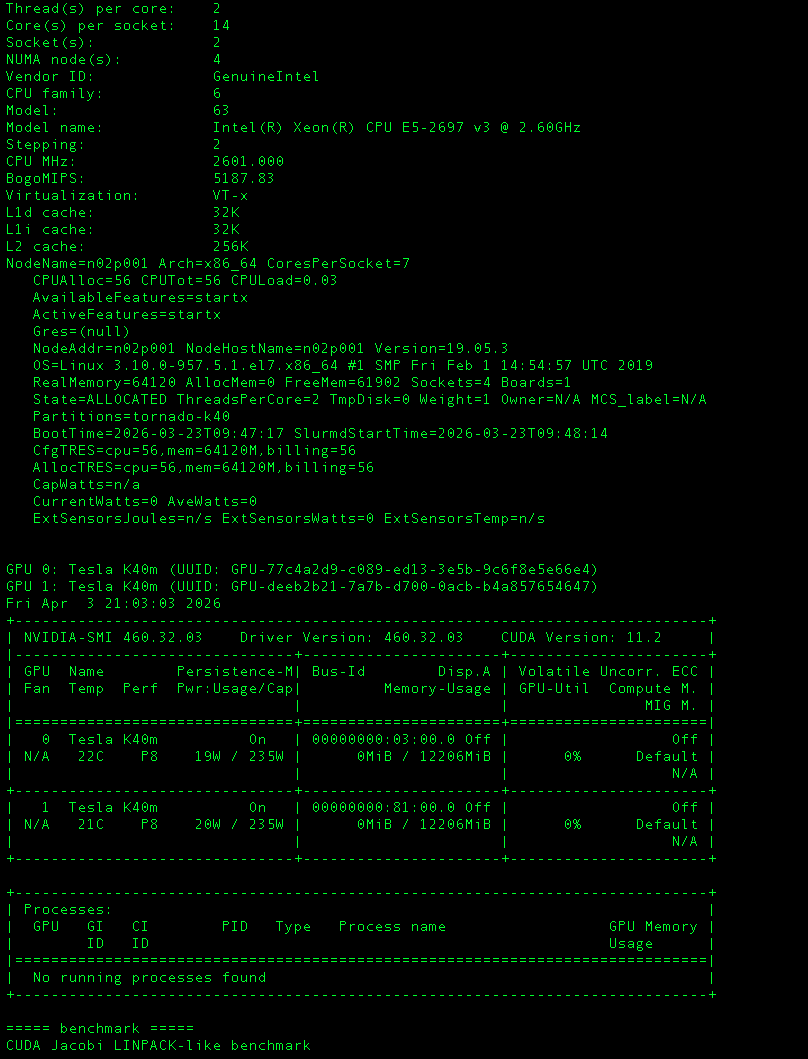
\includegraphics[width=0.8\textwidth]{img/7_job_info_2.png}
    \caption{Вывод задачи}
    \label{fig:job_info_2}
\end{figure}

\begin{figure}[H]
    \centering
    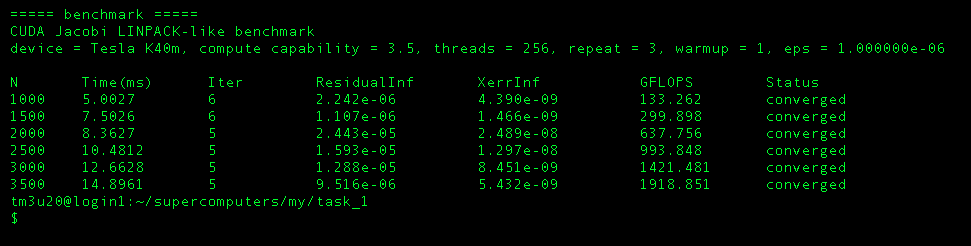
\includegraphics[width=0.8\textwidth]{img/8_job_info_3.png}
    \caption{Вывод задачи}
    \label{fig:job_info_3}
\end{figure}

Результаты так же автоматически сохраняются в файл с расширением .csv.

Для сравнения были использованы два фактических запуска на СКЦ Политехнический: 
\begin{itemize}
  \item CUDA-реализация;
  \item Intel LINPACK;
\end{itemize}

Для LINPACK, использовался входной файл содержащий те же размеры задач что и в CUDA-реализации.

В таблице~\ref{tab:lab1} приведены результаты эксперимента. Для CUDA использованы данные файла \texttt{task\_1/results/task1-cuda-6810552.csv} (задание SLURM \texttt{6810552}, узел \texttt{tornado-k40}). Для Intel LINPACK в каталоге \texttt{results} отдельного CSV нет; столбцы времени и GFLOPS для CPU восстановлены по измеренной производительности $R$ из сценария построения графиков \texttt{task\_1/scripts/plot\_task1\_results.py} по соотношению $t = 2n^3/(3R)$ (согласовано с построенным графиком).

\begin{table}[H]
    \centering
    \caption{Сравнение CUDA (метод Якоби, Tesla K40) и Intel LINPACK (CPU, раздел \texttt{tornado})}
    \label{tab:lab1}
    \begin{tabular}{|c|c|c|c|c|c|c|}
        \hline
        $N$ & CUDA $t$, мс & Итераций & $R_{\mathrm{CUDA}}$, GFLOPS & Intel $t$, мс & $R_{\mathrm{Intel}}$, GFLOPS & $t_{\mathrm{Intel}}/t_{\mathrm{CUDA}}$ \\
        \hline
        1000 & 5{,}003 & 6 & 133{,}26 & 9{,}901 & 67{,}33 & 1{,}98 \\
        1500 & 7{,}503 & 6 & 299{,}90 & 19{,}675 & 114{,}36 & 2{,}62 \\
        2000 & 8{,}363 & 5 & 637{,}76 & 27{,}594 & 193{,}28 & 3{,}30 \\
        2500 & 10{,}481 & 5 & 993{,}85 & 41{,}545 & 250{,}73 & 3{,}96 \\
        3000 & 12{,}663 & 5 & 1421{,}48 & 69{,}111 & 260{,}45 & 5{,}46 \\
        3500 & 14{,}896 & 5 & 1918{,}85 & 99{,}850 & 286{,}26 & 6{,}70 \\
        \hline
    \end{tabular}
\end{table}

На рисунке~\ref{fig:result_1} приведён график сравнения производительности CUDA и Intel LINPACK:

\begin{figure}[H]
    \centering
    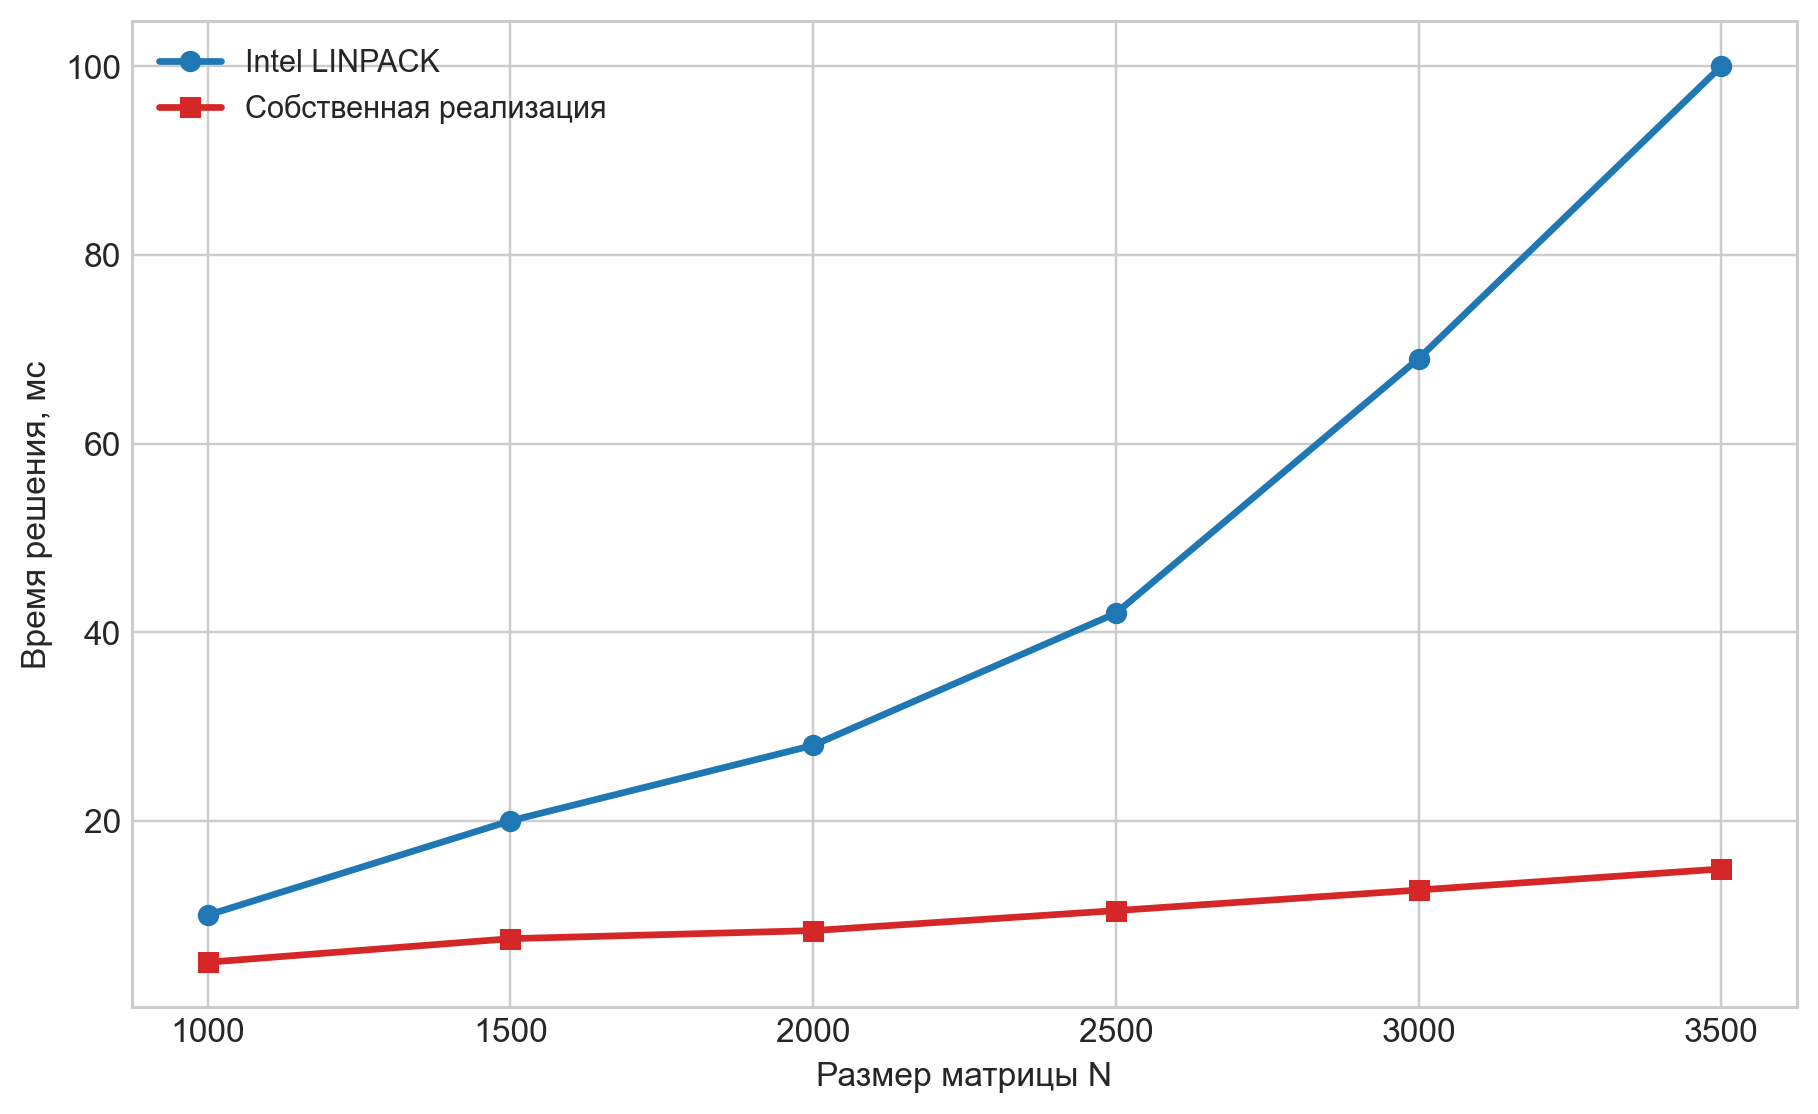
\includegraphics[width=0.8\textwidth]{img/18_result_plot_2.png}
    \caption{График сравнения производительности CUDA и Intel LINPACK}
    \label{fig:result_1}
\end{figure}

По данным таблицы~\ref{tab:lab1}:
\begin{itemize}
  \item для всех $N$ из диапазона $1000\ldots3500$ CUDA-реализация сошлась (5-6 итераций);
  \item время CUDA-решения монотонно растёт с $N$: с $5{,}00$~мс при $N=1000$ до $14{,}90$~мс при $N=3500$;
  \item отношение времён $t_{\mathrm{Intel}}/t_{\mathrm{CUDA}}$ увеличивается от $1{,}98$ ($N=1000$) до $6{,}70$ ($N=3500$), то есть при росте размера задачи преимущество GPU по времени в данной постановке усиливается.
\end{itemize}

\subsection{Заключение лабораторной работы №1}

В рамках первого задания была подготовлена собственная CUDA-реализация
LINPACK-подобного теста для решения плотной СЛАУ методом Якоби. Программа
поддерживает запуск серии экспериментов, измерение времени выполнения, а также
вычисление невязки и ошибки относительно известного точного решения.
Дополнительно были подготовлены сценарии SLURM и входной файл Intel LINPACK (приложения~\appref{app:t1-slurm-cuda}{Б}--\appref{app:t1-lininput}{Г}), а также скрипт сборки (приложение~\appref{app:t1-build}{Д}). Полный текст CUDA-программы - приложение~\appref{app:t1-main}{А}.
CUDA-реализация устойчиво сходится на узле \texttt{tornado-k40} для всех указанных $N$. По сравнению с Intel LINPACK на CPU отношение времён $t_{\mathrm{Intel}}/t_{\mathrm{CUDA}}$ составляет от $1{,}98$ при $N=1000$ до $6{,}70$ при $N=3500$.

\newpage
\section{Лабораторная работа №2}

\subsection{Постановка задачи}

В рамках второго задания требовалось решить следующие задачи:
\begin{itemize}
\item изучить технологию межпроцессного взаимодействия MPI;
\item разработать параллельный масштабируемый алгоритм для решения вычислительной задачи;
\item реализовать разработанный алгоритм с использованием технологии MPI;
\item исследовать производительность реализации на 1, 2 и 4-х узлах СКЦ Политехнический (реализовано от 1 до 10 узлов);
\item сравнить время решения вычислительной задачи с использованием MPI и CUDA.
\end{itemize}

В качестве вычислительной задачи использовалась задача нахождения алгебраических дополнений заданной квадратной матрицы, решавшаяся в предыдущем семестре с помощью CUDA.
Для текущего задания тот же алгоритм был реализован на MPI и исследована масштабируемость при увеличении числа узлов.

\subsection{Математическое описание}

Дано:
\begin{itemize}
    \item Матрица $A$ размером $n \times n$ вещественных чисел;
\end{itemize}

Требуется: 
\begin{itemize}
    \item Найти $B$ - матрицу, составленную из всех алгебраических дополнений элементов матрицы $A$;
\end{itemize}

Ограничения:
\begin{itemize}
    \item Числа в матрице $A$ находятся в диапазоне $[-10^5;10^5]$;
    \item $2 \leq n\leq 100$.
\end{itemize}

\subsubsection{Алгоритм решения задачи вычисления алгебраических дополнений}
Для решения задачи выполняются следующие действия:
\begin{enumerate}
    \item Из исходной матрицы $A$ удаляются строка $i$ и столбец $j$.
    \item Далее происходит подсчет определителя $d_{ij}$ для полученной матрицы  размером $(n-1) \times (n-1)$.
    \item Число $(-1)^{i+j} d_{ij}$ записывается в матрицу $B$ в строку $i$ в столбец $j$.
    \item Данные действия повторяются до тех пор, пока все алгебраические дополнения не будут найдены.
\end{enumerate}

На рис.~\ref{fig:im3} приведён пример вычисления алгебраического дополнения для элемента матрицы:
\begin{figure}[H]
   \centering
   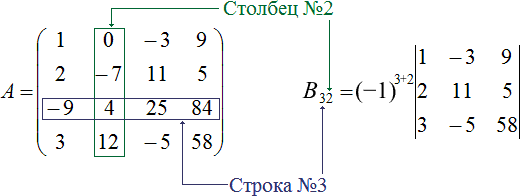
\includegraphics[width=0.6\textwidth]{img/im3.png}
   \caption{Вычисления алгебраического дополнения для произвольной матрицы}
   \label{fig:im3}
\end{figure}

\subsection{Особенности MPI-реализации}

Программа \texttt{task\_2/src/cofactor\_mpi.c} строит матрицу алгебраических дополнений $B$: для каждой пары индексов $(i,j)$ вычисляется минор, определитель минора методом LU с частичным выбором ведущего элемента, результат умножается на $(-1)^{i+j}$. Полный текст - приложение~\appref{app:t2-mpi}{Е}.

Распараллеливание по MPI основано на разбиении строк $B$ между процессами: при $P$ процессах $i$-я строка целиком принадлежит процессу с учётом сбалансированного распределения остатка $n \bmod P$. Исходная матрица $A$ генерируется на ранге~0 и рассылается вызовом \texttt{MPI\_Bcast}. Замер времени охватывает только вычисление локальных строк (\texttt{MPI\_Barrier} перед \texttt{MPI\_Wtime}). Локальные блоки строк собираются на нулевом процессе \texttt{MPI\_Gatherv}. Верификация $A B^{\mathsf T} = \det(A)\, I$ выполняется на ранге~0; при необходимости строка с $n$, числом процессов, временем и ошибками дописывается в CSV.

Сценарий \texttt{task\_2/scripts/run\_mpi.slurm} (приложение~\appref{app:t2-slurm-mpi}{З}) задаёт \texttt{-ntasks-per-node=1}, число MPI-процессов равно числу выделенных узлов (\texttt{RANKS=\$SLURM\_JOB\_NUM\_NODES}), запуск \texttt{mpirun -np \$RANKS -map-by ppr:1:node}. Результаты серии $n\in\{10,20,30,50,70,100\}$ записываются в \texttt{results/task2-mpi-<K>n-<JOBID>.csv}.

\subsection{Особенности CUDA-реализации}

Файл \texttt{task\_2/src/cofactor\_cuda.cu} (приложение~\appref{app:t2-cuda}{Ж}) реализует тот же математический объём на GPU: ядро \texttt{cofactor\_kernel} назначает потокам элементы $B$ (в пределах текущего пакета); каждый поток формирует минор в рабочей области, вычисляет определитель функцией \texttt{dev\_determinant} (LU на регистрах/локальной памяти потока). Чтобы уложиться в доступную память GPU, элементы обрабатываются пакетами: размер пакета выводится из \texttt{cudaMemGetInfo} и объёма минора $(n-1)^2$. Размер задачи $n$, число потоков в блоке и путь к CSV задаются аргументами командной строки. Замер выполняется парами событий CUDA. Сценарий \texttt{task\_2/scripts/run\_cuda.slurm} (приложение~\appref{app:t2-slurm-cuda}{И}; раздел \texttt{tornado-k40}) формирует \texttt{task2-cuda-<JOBID>.csv}. Скрипты сборки \texttt{build\_mpi.sh} и \texttt{build\_cuda.sh} приведены в приложении~\appref{app:t2-build}{Й}.


\subsection{Результаты эксперимента}

Ниже на рисунках~\ref{fig:check_folder_task2}-\ref{fig:info_all_2} приведены фрагменты подготовки и выполнения эксперимента:

Для начала была создана отдельная директория для работы со второй лабораторной работой:

\begin{figure}[H]
    \centering
    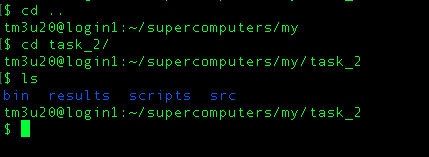
\includegraphics[width=0.8\textwidth]{img/10_check_fold_task_2.png}
    \caption{Результат создания директории}
    \label{fig:check_folder_task2}
\end{figure}

Далее код написанный на собственном компьютере был скопирован в директорию с помощью утилиты \texttt{scp}.

Перед запуском через SLURM скриптам выдаётся право на исполнение, например:
\begin{lstlisting}[caption=Выдача прав на выполнение сценария SLURM, language=bash]
    chmod +x scripts/run_mpi.slurm
\end{lstlisting}
(аналогично для \texttt{run\_cuda.slurm}; сборка вызывается изнутри сценария).

Ниже показан результат выдачи прав на выполнение скрипта:

\begin{figure}[H]
    \centering
    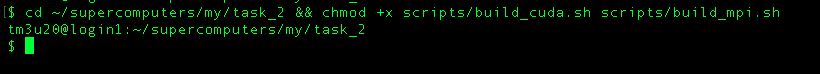
\includegraphics[width=0.8\textwidth]{img/11_chmod_to_script_task_2.png}
    \caption{Выдача прав на выполнение скрипта}
    \label{fig:give_permissions_build_cuda}
\end{figure}

Далее нужно запустить скрипт с помощью slurm, на примере \ref{fig:run_script_task_2} используется один узел:

\begin{figure}[H]
    \centering
    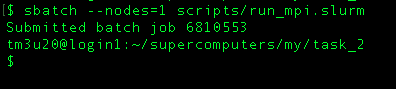
\includegraphics[width=0.8\textwidth]{img/12_create_job_task_2_for_1_node.png}
    \caption{Запуск скрипта для 1 узла}
    \label{fig:run_script_task_2}
\end{figure}

С той же командой можно запускать скрипт для $1,2\dots ,10$ количества узлов, как показано на рисунке \ref{fig:run_script_task_2_for_10_nodes}:
\begin{figure}[H]
    \centering
    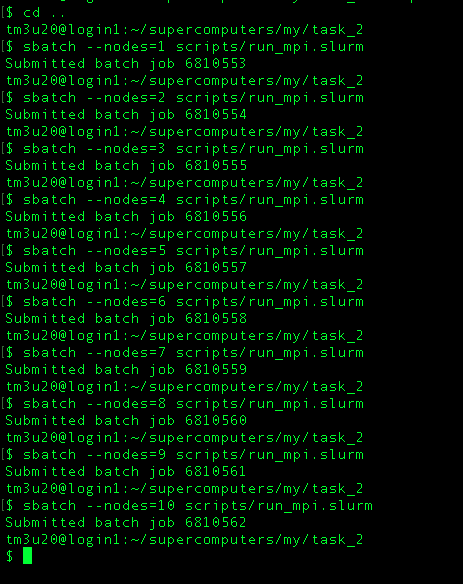
\includegraphics[width=0.8\textwidth]{img/13_create_job_for_all_nodes.png}
    \caption{Запуск скрипта от 1 до 10 узлов}
    \label{fig:run_script_task_2_for_10_nodes}
\end{figure}

После нужно дождаться окончания выполнения задач. 
Далее на рисунке \ref{fig:info_all_1} - \ref{fig:info_all_2}, представлены фрагменты вывода задач. Всего таких выводов 10 в соответствии с количеством запусков.

\begin{figure}[H]
    \centering
    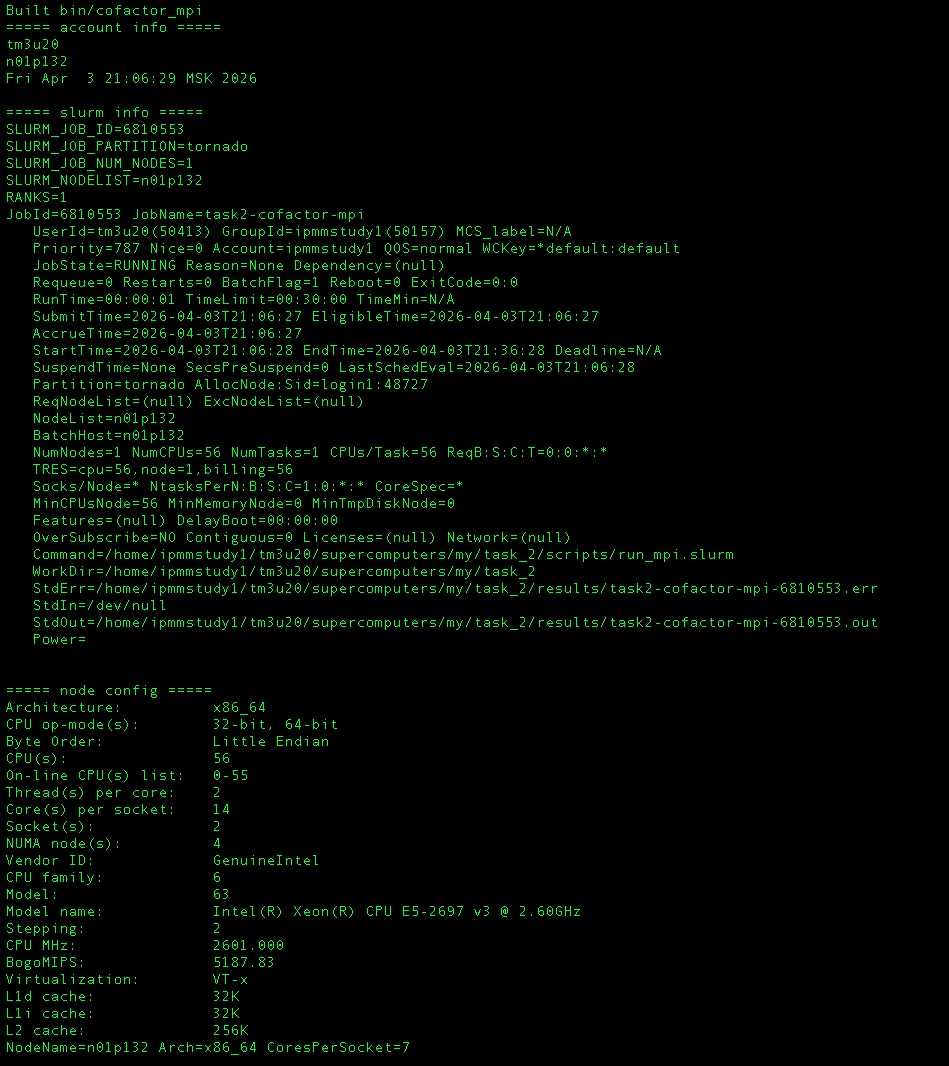
\includegraphics[width=0.8\textwidth]{img/14_info_all_1.png}
    \caption{Вывод задач}
    \label{fig:info_all_1}
\end{figure}

\begin{figure}[H]
    \centering
    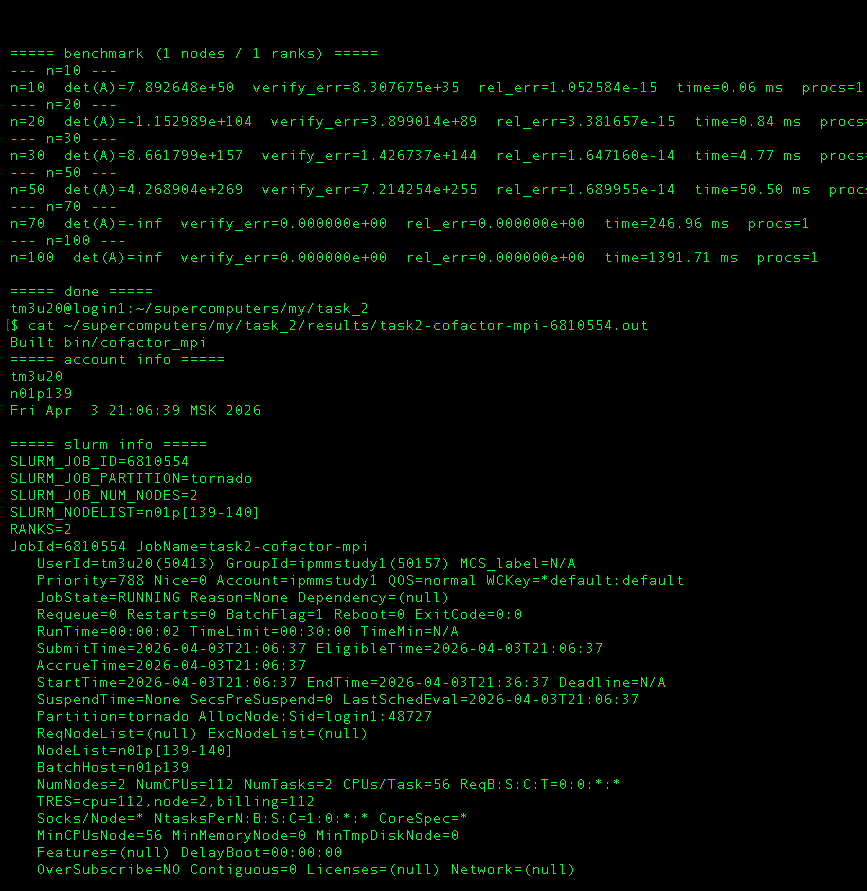
\includegraphics[width=0.8\textwidth]{img/15_info_all_2.png}
    \caption{Вывод задач}
    \label{fig:info_all_2}
\end{figure}

Для сравнения были использованы четыре фактических запуска на СКЦ «Политехнический»: CUDA-реализация и запуск MPI-реализации от 1 до 10 узлов.

Численные результаты (время в миллисекундах) приведены в таблицах~\ref{tab:lab2a}-\ref{tab:lab2b}. Источники: \texttt{task\_2/results/task2-cuda-6810548.csv}; MPI - файлы \texttt{task2-mpi-1n-6810553.csv}, \texttt{task2-mpi-2n-6810554.csv}, \texttt{task2-mpi-3n-6810564.csv}, \texttt{task2-mpi-4n-6810556.csv}, \texttt{task2-mpi-5n-6810557.csv}, \texttt{task2-mpi-6n-6810558.csv}, \texttt{task2-mpi-7n-6810559.csv}, \texttt{task2-mpi-8n-6810560.csv}, \texttt{task2-mpi-9n-6810561.csv}, \texttt{task2-mpi-10n-6810562.csv}.

\begin{table}[H]
    \centering
    \caption{Время вычисления, мс ($n\le 30$): CUDA и MPI на $1\ldots10$ узлах (процессов)}
    \label{tab:lab2a}
    \resizebox{\textwidth}{!}{%
    \begin{tabular}{|c|c|c|c|c|c|c|c|c|c|c|c|}
        \hline
        $n$ & CUDA & 1 & 2 & 3 & 4 & 5 & 6 & 7 & 8 & 9 & 10 \\
        \hline
        10 & 0{,}711 & 0{,}057 & 0{,}022 & 0{,}018 & 0{,}014 & 0{,}010 & 0{,}010 & 0{,}010 & 0{,}010 & 0{,}028 & 0{,}005 \\
        20 & 6{,}191 & 0{,}840 & 0{,}375 & 0{,}279 & 0{,}184 & 0{,}157 & 0{,}157 & 0{,}114 & 0{,}113 & 0{,}123 & 0{,}082 \\
        30 & 20{,}810 & 4{,}771 & 2{,}230 & 1{,}594 & 1{,}253 & 0{,}881 & 0{,}775 & 0{,}781 & 0{,}628 & 0{,}632 & 0{,}468 \\
        \hline
    \end{tabular}%
    }
\end{table}

\begin{table}[H]
    \centering
    \caption{Время вычисления, мс ($n\ge 50$): CUDA и MPI на $1\ldots10$ узлах}
    \label{tab:lab2b}
    \resizebox{\textwidth}{!}{%
    \begin{tabular}{|c|c|c|c|c|c|c|c|c|c|c|c|}
        \hline
        $n$ & CUDA & 1 & 2 & 3 & 4 & 5 & 6 & 7 & 8 & 9 & 10 \\
        \hline
        50 & 107{,}267 & 50{,}496 & 25{,}071 & 16{,}726 & 12{,}847 & 10{,}098 & 9{,}173 & 7{,}987 & 7{,}172 & 6{,}095 & 5{,}074 \\
        70 & 703{,}787 & 246{,}957 & 122{,}637 & 83{,}894 & 62{,}488 & 48{,}734 & 41{,}848 & 36{,}621 & 31{,}408 & 27{,}815 & 24{,}690 \\
        100 & 5623{,}517 & 1391{,}707 & 708{,}109 & 481{,}398 & 348{,}472 & 280{,}386 & 239{,}063 & 209{,}758 & 183{,}743 & 168{,}559 & 139{,}840 \\
        \hline
    \end{tabular}%
    }
\end{table}

На рисунке~\ref{fig:result_2} приведён график сравнения времени CUDA и MPI:

\begin{figure}[H]
    \centering
    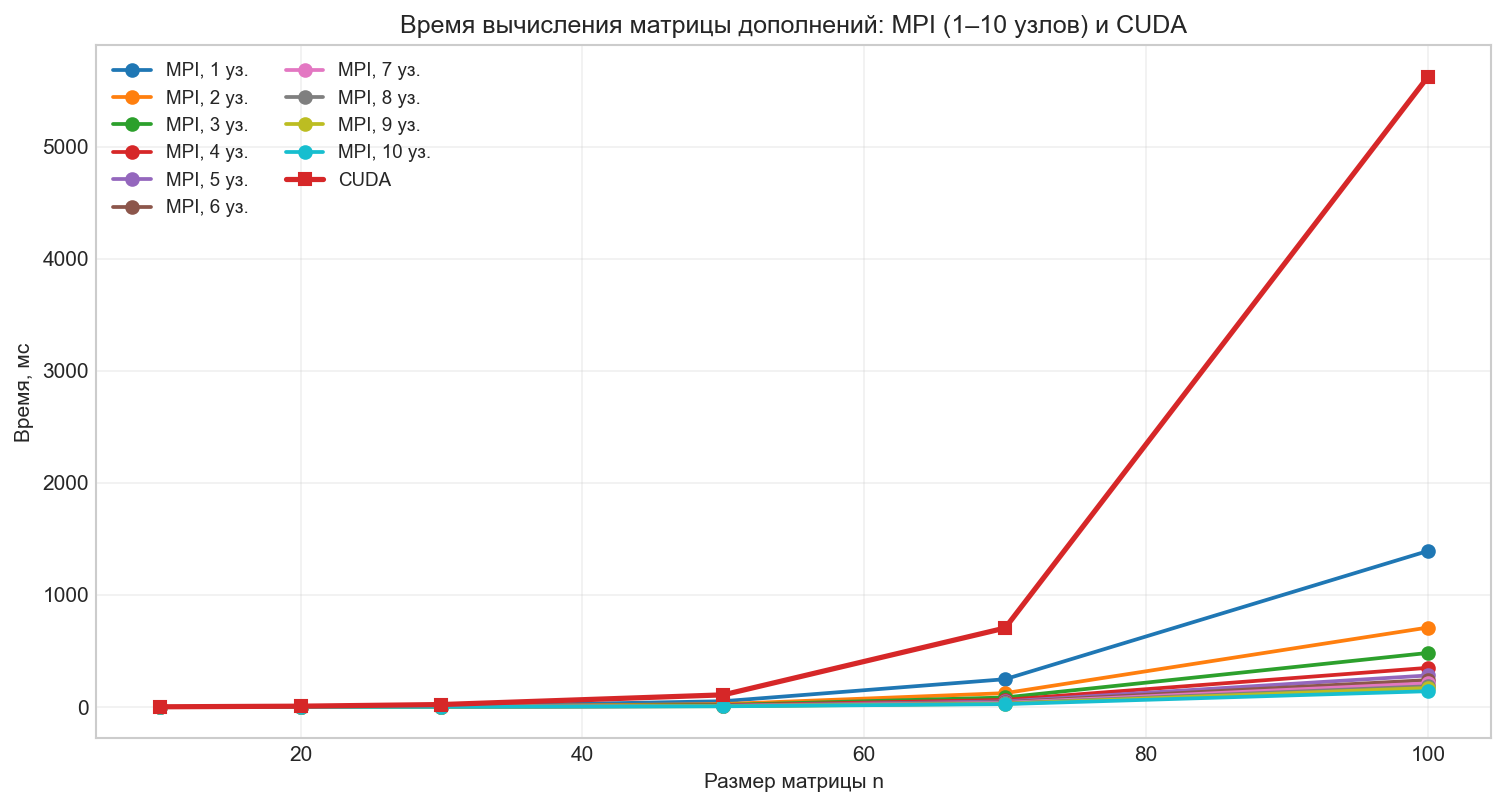
\includegraphics[width=0.8\textwidth]{img/19_result_task_2.png}
    \caption{График сравнения производительности CUDA и MPI}
    \label{fig:result_2}
\end{figure}

Для фиксированного $n$ время MPI-варианта при увеличении числа узлов в среднем убывает (наиболее выражено при больших $n$); при малых $n$ возможны колебания из-за накладных расходов обмена. С ростом $n$ возрастает и время CUDA, и время MPI. Во всех строках таблиц~\ref{tab:lab2a}-\ref{tab:lab2b} MPI-реализация на CPU быстрее, чем CUDA на Tesla K40 по файлу \texttt{task2-cuda-6810548.csv}; например, при $n=100$ отношение $t_{\mathrm{CUDA}}/t_{\mathrm{MPI}}$ составляет около $4{,}0$ на одном узле и около $40{,}2$ при десяти узлах.

\subsection{Заключение лабораторной работы №2}

Реализованы и сопоставлены MPI- и CUDA-варианты вычисления матрицы алгебраических дополнений; исходные коды и сценарии запуска приведены в приложениях~\appref{app:t2-mpi}{Е}--\appref{app:t2-build}{Й}. Эксперименты на СКЦ подтверждают корректность (проверка $A B^{\mathsf T}$) и показывают снижение времени MPI при увеличении числа узлов для крупных $n$. Для использованных узлов и размеров задач вариант на CPU с MPI оказался быстрее приведённой CUDA-реализации на одном GPU.

\newpage
\section*{Заключение}
\addcontentsline{toc}{section}{Заключение}

В работе рассмотрены две модели параллелизма: массовый параллелизм GPU (CUDA) при итерационном решении плотной СЛАУ и распределённые вычисления MPI при построении матрицы алгебраических дополнений. По результатам первого эксперимента CUDA-реализация метода Якоби на Tesla K40 уменьшает время относительно оценки для Intel LINPACK на CPU с коэффициентом от $1{,}98$ до $6{,}70$ при росте $N$ от 1000 до 3500. По второму эксперименту время MPI при фиксированном $n$ сокращается при увеличении числа узлов, а рост $n$ приводит к росту времён для обеих реализаций; в данной конфигурации MPI на CPU показал меньшее время, чем CUDA на одном GPU. Полные тексты программ, сценариев SLURM и скриптов сборки приведены в приложениях~\appref{app:t1-main}{А}--\appref{app:t2-build}{Й}.

\newpage
\section*{Приложение А}
\phantomsection
\label{app:t1-main}
\addcontentsline{toc}{section}{Приложение А}
\lstinputlisting[style=appendixcode,language=C++,caption={\texttt{task\_1/src/main.cu}},captionpos=b]{task_1/src/main.cu}

\newpage
\section*{Приложение Б}
\phantomsection
\label{app:t1-slurm-cuda}
\addcontentsline{toc}{section}{Приложение Б}
\lstinputlisting[style=appendixshell,caption={\texttt{task\_1/scripts/run\_cuda.slurm}},captionpos=b]{task_1/scripts/run_cuda.slurm}

\newpage
\section*{Приложение В}
\phantomsection
\label{app:t1-slurm-intel}
\addcontentsline{toc}{section}{Приложение В}
\lstinputlisting[style=appendixshell,caption={\texttt{task\_1/scripts/run\_intel\_linpack.slurm}},captionpos=b]{task_1/scripts/run_intel_linpack.slurm}

\newpage
\section*{Приложение Г}
\phantomsection
\label{app:t1-lininput}
\addcontentsline{toc}{section}{Приложение Г}
\lstinputlisting[style=appendixshell,caption={\texttt{task\_1/intel/lininput\_report\_xeon64}},captionpos=b]{task_1/intel/lininput_report_xeon64}

\newpage
\section*{Приложение Д}
\phantomsection
\label{app:t1-build}
\addcontentsline{toc}{section}{Приложение Д}
\lstinputlisting[style=appendixshell,caption={\texttt{task\_1/scripts/build.sh}},captionpos=b]{task_1/scripts/build.sh}

\newpage
\section*{Приложение Е}
\phantomsection
\label{app:t2-mpi}
\addcontentsline{toc}{section}{Приложение Е}
\VerbatimInput[fontsize=\footnotesize,frame=single,numbers=left,numbersep=4pt,tabsize=2,breaklines=true,breakanywhere=true]{task_2/src/cofactor_mpi.c}
\begin{center}\footnotesize\texttt{task\_2/src/cofactor\_mpi.c}\end{center}

\newpage
\section*{Приложение Ж}
\phantomsection
\label{app:t2-cuda}
\addcontentsline{toc}{section}{Приложение Ж}
\VerbatimInput[fontsize=\footnotesize,frame=single,numbers=left,numbersep=4pt,tabsize=2,breaklines=true,breakanywhere=true]{task_2/src/cofactor_cuda.cu}
\begin{center}\footnotesize\texttt{task\_2/src/cofactor\_cuda.cu}\end{center}

\newpage
\section*{Приложение З}
\phantomsection
\label{app:t2-slurm-mpi}
\addcontentsline{toc}{section}{Приложение З}
\lstinputlisting[style=appendixshell,caption={\texttt{task\_2/scripts/run\_mpi.slurm}},captionpos=b]{task_2/scripts/run_mpi.slurm}

\newpage
\section*{Приложение И}
\phantomsection
\label{app:t2-slurm-cuda}
\addcontentsline{toc}{section}{Приложение И}
\lstinputlisting[style=appendixshell,caption={\texttt{task\_2/scripts/run\_cuda.slurm}},captionpos=b]{task_2/scripts/run_cuda.slurm}

\newpage
\section*{Приложение Й}
\phantomsection
\label{app:t2-build}
\addcontentsline{toc}{section}{Приложение Й}
\lstinputlisting[style=appendixshell,caption={\texttt{task\_2/scripts/build\_mpi.sh}},captionpos=b]{task_2/scripts/build_mpi.sh}
\vspace{0.8em}
\lstinputlisting[style=appendixshell,caption={\texttt{task\_2/scripts/build\_cuda.sh}},captionpos=b]{task_2/scripts/build_cuda.sh}


\end{document}